\documentclass[12pt,a4paper,oneside]{TechnicalDocumentation}

\usepackage{times}
\usepackage{graphicx}
\usepackage{float}
\usepackage{tabularx}
\usepackage{placeins}
\usepackage{caption}
\usepackage{geometry}
\usepackage{enumitem}
\usepackage{hyperref}
\usepackage[most]{tcolorbox}

\geometry{left=2cm,right=2cm,top=2cm,bottom=2.5cm}
\graphicspath{{./Images/}{./Images/assembly_copilot/}}
\tcbset{arc=0mm, colback=darkBlue!5!white, boxrule=0.3mm, colframe=black}
\setlist{itemsep=2pt, topsep=3pt}
\renewcommand{\arraystretch}{1.18}

\hypersetup{
    hidelinks,
    pdftitle={Assembly Copilot: Procedure Step Recognition from Research to Operational Demonstration},
    pdfauthor={AIOPS Team}
}

\begin{document}

\coverpage
{Assembly Copilot: Procedure Step Recognition from Research to Operational Demonstration}
{}
{Technical Documentation}
{2026}
{Images/LM-logo-Black.png}

\tableofcontents

\chapter{Preface}

\section{Project Description}

Assembly Copilot is a computer-vision system that observes an operator's
egocentric video while an assembly procedure is being performed. It estimates
which procedure step is currently in progress, announces completed steps, and
surfaces out-of-order activity for review. The project connects procedure-step
recognition research with a working demonstration that can be replayed in a
browser, served through a live video path, and displayed on a HoloLens overlay.

The demonstrator uses a ten-part turbofan engine model as the assembly object.
The model is deliberately small enough to support rapid experimentation while
retaining the practical characteristics of a production task: hand-object
occlusion, similar-looking parts, variable step duration, incomplete views, and
operators who do not follow exactly the same order.

\section{Project Value}

The intended value is an additional source of situational awareness for an
operator or supervisor. A live system can reduce the need to manually track
procedure progress, make deviations visible earlier, and provide a consistent
record for post-task review. The system is an assistive demonstrator; it is not
a replacement for approved work instructions, inspection, or human sign-off.

\section{Documentation Scope}

This document records the development path from preliminary procedure-step
recognition experiments to the current live inference demonstration. It covers
the project objective, data collection and labeling tools, model development,
streaming inference, application presentation, HoloLens integration, measured
results, limitations, and recommended next steps. Proprietary internal model
implementation details are described at the level needed to understand the
system behavior and engineering decisions.

\section{Key Outcomes}

\begin{table}[H]
\centering
\small
\begin{tabularx}{\textwidth}{@{}p{0.22\textwidth}X@{}}
\toprule
\textbf{Area} & \textbf{Documented outcome} \\
\midrule
Research & Controlled progression from a VideoMAEv2 baseline to a fused
motion-and-appearance model with the best IndustReal result. \\
Data & Own egocentric engine-model recordings, dense labels, and stress
variants for normal and non-nominal procedure behavior. \\
Deployment & Causal temporal inference with fixed-lag commitment, replay and
live services, and a HoloLens presentation path. \\
Evidence & Separate offline, online, robustness, latency, and interface
evidence so the demonstrator is not represented by one number alone. \\
\bottomrule
\end{tabularx}
\caption{Summary of the project outcomes covered in this document.}
\label{tab:key-outcomes}
\end{table}

\chapter{Program Context and Objective}

\section{Operational Problem}

Assembly is a time-dependent process. The operator may hold a part out of view,
repeat a motion, pause, or perform a valid operation in a different order from
another operator. A useful vision system therefore has to interpret a sequence
of observations rather than classify isolated images. It must also make a
decision from the video available so far; using future frames would make an
offline result look stronger than a real deployment can be.

The project objective was to build that complete chain: capture representative
egocentric video, label the procedure, evaluate candidate recognition approaches,
adapt the strongest feature representation to causal inference, and expose the
result through interfaces suitable for demonstration.

\section{Development Objectives}

\begin{enumerate}
    \item Establish a repeatable procedure-step recognition workflow using the
    IndustReal research setting.
    \item Collect and label an in-house egocentric dataset on the turbofan
    engine model.
    \item Compare model architectures, visual representations, temporal
    modeling, and decoding choices using consistent metrics.
    \item Train and validate a streaming model that does not inspect future
    frames.
    \item Demonstrate the result through replay, live video, and a wearable
    HoloLens interface.
\end{enumerate}

\section{Scope Boundaries and Success Criteria}

The project was scoped as a procedure-state assistant, not as a complete
factory inspection system. The target behavior was to identify the part or
procedure state visible in the egocentric stream, preserve the order and
duration of the recognized steps, and expose a stable result with enough
latency and robustness for a live demonstration. It was not intended to
replace an approved work instruction, determine torque or fit, certify a
completed installation, or independently authorize an operator to continue.

Progress was evaluated at three levels. Research experiments had to show a
measurable improvement in temporal recognition quality. The own-dataset phase
had to produce repeatable labels, held-out evaluation, and stress cases that
challenged memorized procedure order. The final demonstration had to connect
the model to a functioning replay path, a live stream, and a wearable
presentation. This staged definition prevented a high offline score from being
treated as sufficient evidence of operational readiness.

\section{Development Path}

\begin{table}[H]
\centering
\small
\begin{tabularx}{\textwidth}{@{}p{0.22\textwidth}X@{}}
\toprule
\textbf{Stage} & \textbf{Outcome} \\
\midrule
PSR research & Baselines and controlled experiments on IndustReal established
the useful combination of motion and appearance information. \\
Own data collection & Forty curated egocentric recordings were captured on a
ten-part engine model, covering assembly and disassembly. \\
Annotation and stress testing & Dense completion labels were produced and
additional recordings were generated for scrambled, reversed, partial, and
wrong-step behavior. \\
Streaming conversion & Offline sequence modeling was converted to a causal
temporal model with a fixed-lag decoder. \\
Operational demonstration & Replay and live services were connected to a
browser interface and a HoloLens overlay. \\
\bottomrule
\end{tabularx}
\caption{Project progression from research to demonstration.}
\label{tab:development-path}
\end{table}

\section{Transition from Research to the Own Dataset}

The IndustReal experiments selected the feature and temporal-modeling direction;
they did not replace the need for an internal dataset. The engine-model
recordings were collected to test the selected approach under the camera
perspective, part vocabulary, lighting, operator behavior, and procedure
variability relevant to the intended demonstration. This transition is
important: the project moved from comparing architectures on a benchmark to
building a complete data-to-deployment loop in which recording, annotation,
training, evaluation, replay, and live presentation could all be controlled by
the project team.

\section{Assembly Object}

\begin{figure}[H]
\centering
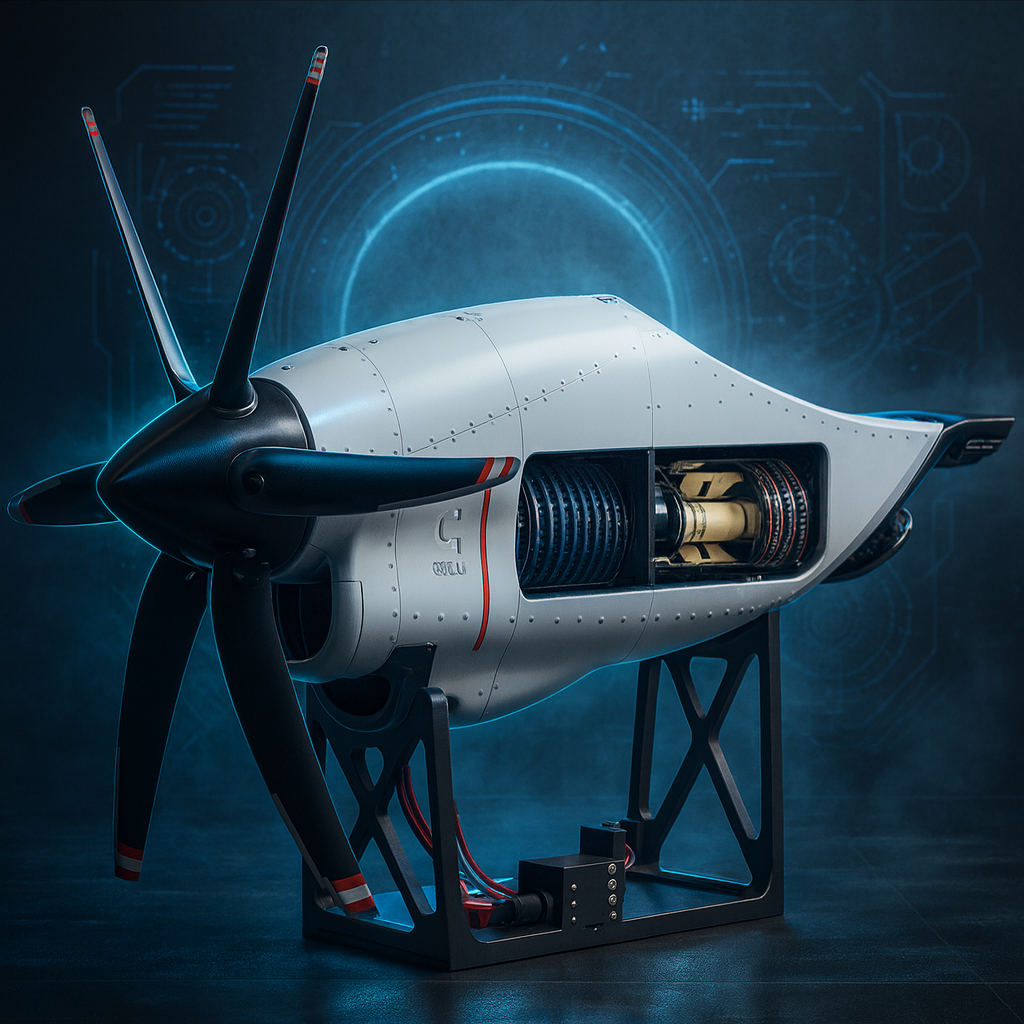
\includegraphics[width=0.72\textwidth]{engine_model_reference.png}
\caption{The turbofan engine model used for the project dataset and
demonstration.}
\label{fig:engine-model}
\end{figure}

The model provides ten named parts and supports both installation and removal
procedures. The visual appearance of a part is only one cue: the system must
also use motion, temporal context, and the state of the procedure to determine
which step is taking place.

\section{System Boundary at the Demonstration Handoff}

\begin{table}[H]
\centering
\small
\begin{tabularx}{\textwidth}{@{}X X@{}}
\toprule
\textbf{Within the demonstrated scope} & \textbf{Outside the demonstrated
scope} \\
\midrule
Recognizing a procedure state from egocentric video. &
Certifying torque, fit, or final installation quality. \\
Committing stable steps and showing procedure progress. &
Replacing approved work instructions or human sign-off. \\
Flagging out-of-order or attention-requiring activity. &
Providing a complete fault taxonomy for every assembly failure. \\
Delivering state to replay, live, and wearable interfaces. &
Spatially anchoring every instruction to a physical part. \\
\bottomrule
\end{tabularx}
\caption{Capability boundary used to interpret the current demonstration.}
\label{tab:scope-boundary}
\end{table}

\chapter{Model Architecture}
\label{ch:model-architecture}

\section{Offline v4 Research Architecture}

The offline v4 system was the strongest research configuration before the
project moved from the IndustReal benchmark to the internally collected
engine-model dataset. It established the representation that was retained in
the later deployment: two complementary, frozen video encoders whose outputs
are normalized and fused. Its temporal and correctness heads, however, were
designed for complete recordings and could use context from both sides of a
transition. It was therefore an important research reference and an upper
bound, rather than the final live architecture.

\begin{figure}[H]
\centering
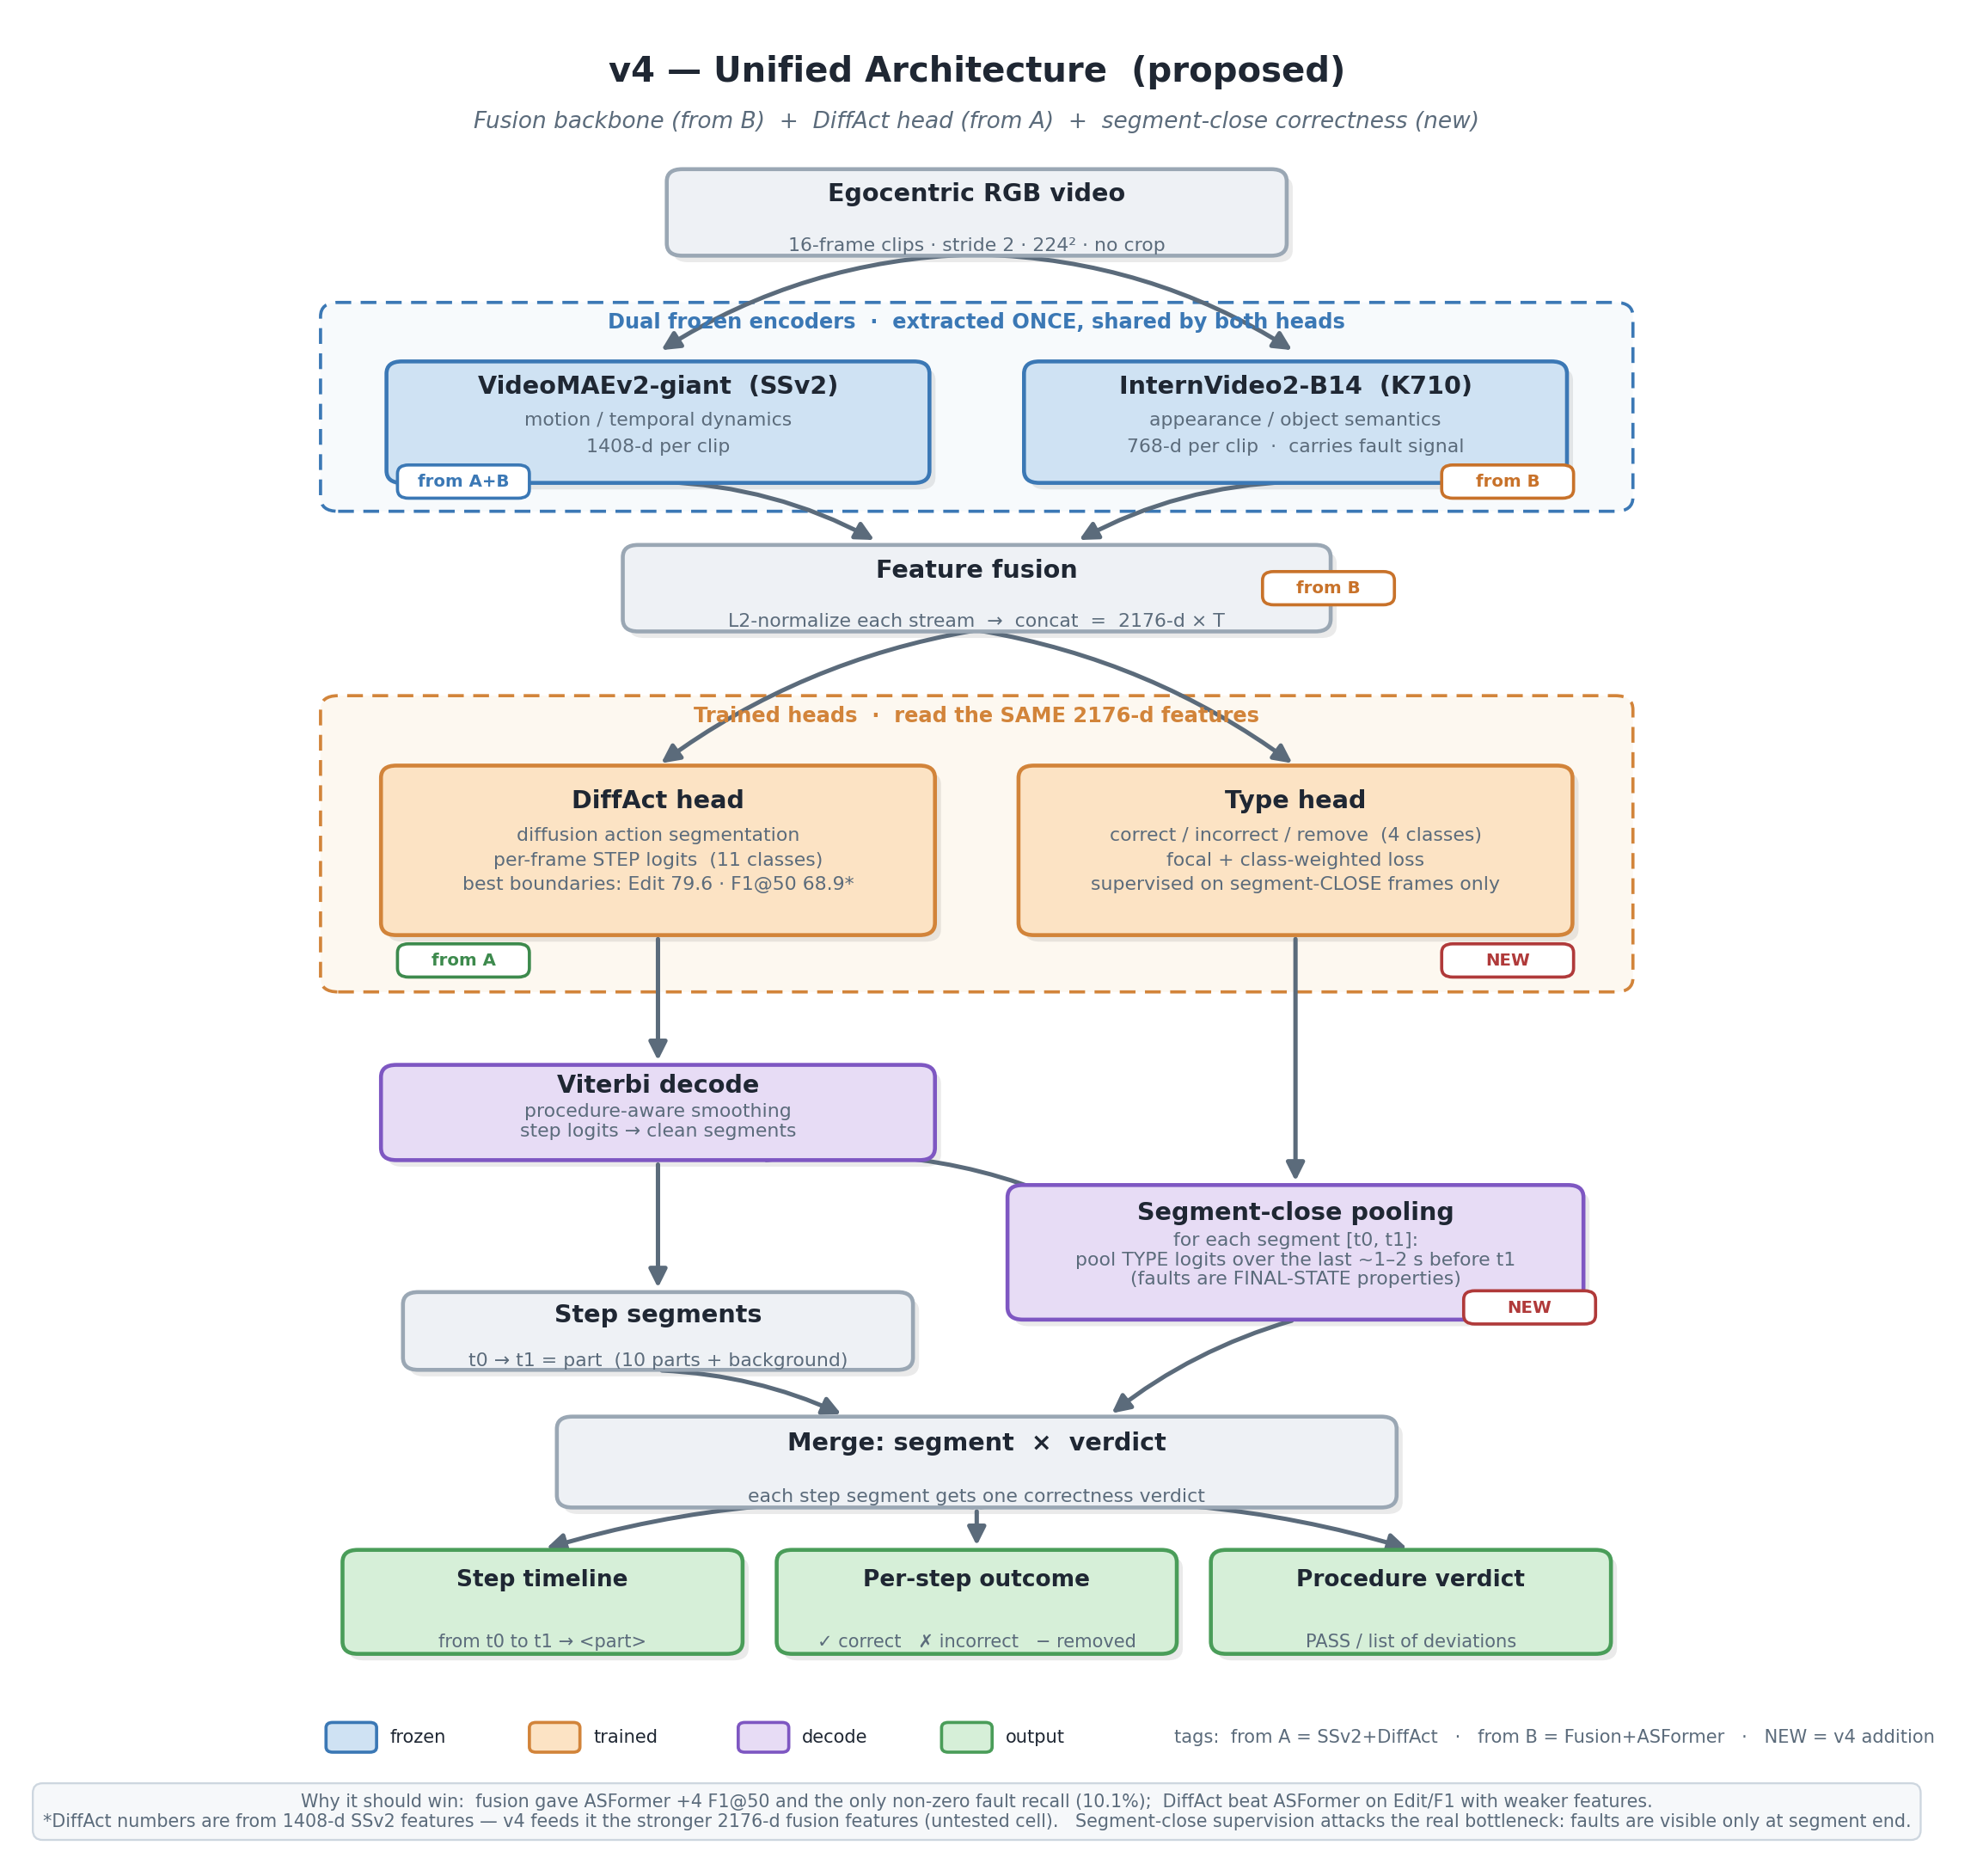
\includegraphics[width=0.88\textwidth]{architecture_v4.png}
\caption{Offline v4 research architecture: fused motion and appearance
features feed the DiffAct segmentation head, type reasoning, and Viterbi
decoding before segment-level outcomes are produced.}
\label{fig:offline-v4-architecture}
\end{figure}

The offline pipeline can be read from left to right. VideoMAEv2-giant provides
the motion-sensitive representation and InternVideo2-B14 provides a
complementary appearance representation. Their 1,408- and 768-dimensional
outputs form a 2,176-dimensional sequence feature. DiffAct predicts the
temporal action structure, while the type head provides an additional signal
for segment interpretation. Viterbi decoding then imposes temporal
consistency and closes segments before a verdict is emitted.

\begin{table}[H]
\centering
\small
\begin{tabularx}{\textwidth}{@{}p{0.32\textwidth}X@{}}
\toprule
\textbf{Offline component} & \textbf{Purpose} \\
\midrule
VideoMAEv2-giant & Frozen motion and temporal-dynamics representation; 1,408
dimensions per clip. \\
InternVideo2-B14 & Frozen appearance and object-semantic representation; 768
dimensions per clip. \\
Feature fusion & L2-normalize both streams and concatenate them into a
2,176-dimensional sequence feature. \\
DiffAct head & Offline action-segmentation head producing per-frame step
logits and strong segment-boundary evidence. \\
Type head and segment close & Exploratory correctness/type reasoning aggregated
over a completed segment instead of trusted from a single frame. \\
Viterbi decode & Procedure-aware smoothing that converts step evidence into
clean, temporally consistent segments. \\
\bottomrule
\end{tabularx}
\caption{Functional elements of the offline v4 research architecture.}
\label{tab:offline-v4-components}
\end{table}

\clearpage
\section{Final Online Deployed Architecture}

The final online architecture preserves the v4 frozen encoders and the
2,176-dimensional fused representation, but changes the temporal decision
path to satisfy the live-inference constraint. The non-streaming DiffAct head
is replaced by a causal temporal convolutional network (TCN), and the
sequence decoder operates with a fixed lag. Every stage sees only past and
present observations; no future frames are used to revise a decision already
delivered to the operator.

\begin{figure}[H]
\centering
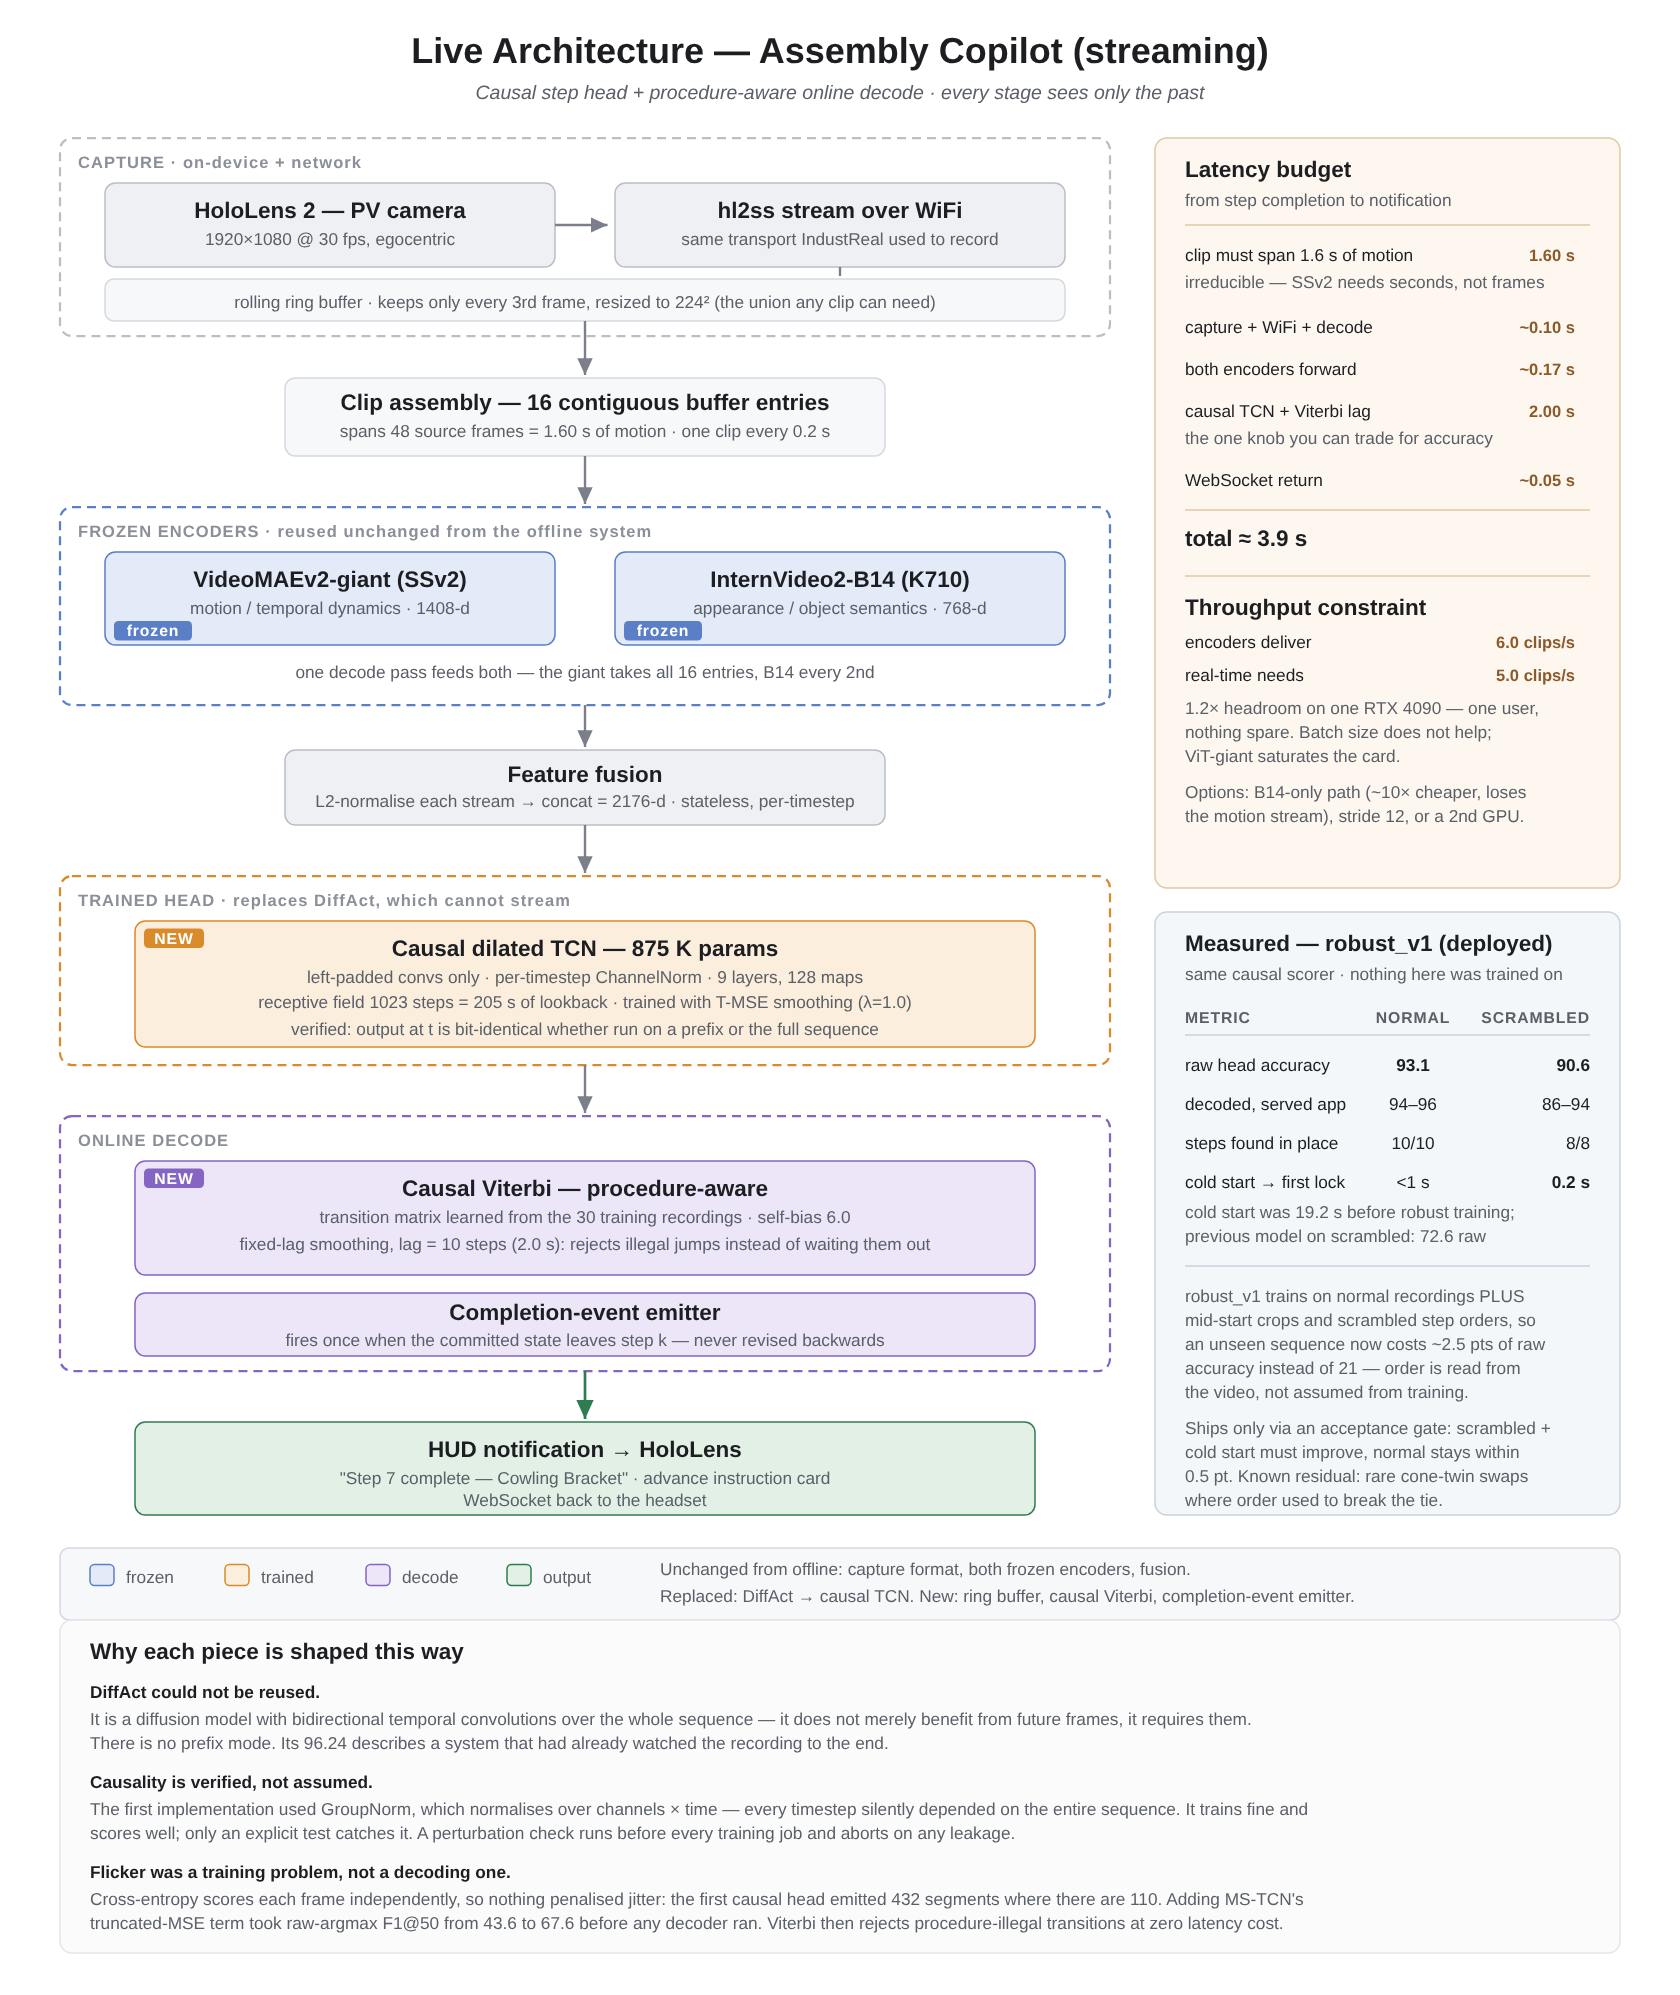
\includegraphics[width=\textwidth]{architecture_live_current.png}
\caption{Final online deployed architecture: camera or HoloLens capture,
rolling clips, frozen encoders, causal temporal scoring, fixed-lag decoding,
and a completion event consumed by the operator interfaces.}
\label{fig:online-architecture}
\end{figure}

\clearpage
\section{Data and Timing at Inference}

The online path is deliberately event-oriented. The classifier produces a
score distribution at every update, but the application does not announce a
new step for every changing score. The decoder maintains a short history,
selects a stable path, and emits a completion event only when the committed
state changes. This separates frequent model updates from the less frequent
operator-facing events used by the replay dashboard and HoloLens overlay.

\begin{table}[H]
\centering
\small
\begin{tabularx}{\textwidth}{@{}p{0.33\textwidth}X@{}}
\toprule
\textbf{Stage} & \textbf{Role in the live system} \\
\midrule
Frame sampling & The source is reduced to approximately 10 frames per second
to make the input rate predictable. \\
Clip construction & Sixteen sampled frames form a 1.6-second clip. A new clip
is evaluated every 0.2 seconds, creating overlapping temporal context. \\
Motion and appearance & VideoMAEv2-giant supplies 1,408 dimensions and
InternVideo2-B14 supplies 768 dimensions; the streams are fused to 2,176
dimensions. \\
Temporal head & A nine-block causal TCN with 128 feature maps models how the
procedure evolves without looking ahead. \\
Decoder and emitter & Fixed-lag Viterbi uses a ten-update, approximately
two-second lag; a step is announced only after the committed state changes. \\
\bottomrule
\end{tabularx}
\caption{Data flow and timing of the final online architecture.}
\label{tab:architecture-stages}
\end{table}

\section{Why the Online Architecture Is Causal}

Offline action-segmentation models can use context on both sides of a
transition. That is useful for research measurement but unavailable when a
technician is being assisted in real time. The causal TCN scores only the
evidence available up to the current update. The decoder delays the commitment
slightly so that a brief occlusion or hand movement does not cause the
interface to announce a false transition.

The measured live announcement delay is approximately 2.84 seconds. It
combines the 1.6-second clip span, the fixed-lag decoder, and processing and
transport time. The final class set contains eleven states: ten named
engine-model parts and a background state; only a committed state change is
treated as a new procedure step.

\section{Model Output}

The model produces a score for each state at every update. The application
compares the newly committed state with the previously committed state. Only a
committed state change is treated as a new procedure step. This distinction
allows the interfaces to refresh continuously while displaying stable current
step and progress information.

\chapter{System Overview and Architecture}

\section{End-to-End Workflow}

The deployed path is organized as a sequence of separable stages:

\begin{enumerate}
    \item A wearable or phone camera supplies an egocentric video stream.
    \item Frames are sampled and grouped into short overlapping clips.
    \item Two frozen video encoders convert each clip into complementary
    motion and appearance features.
    \item The fused features are processed by a causal temporal model.
    \item A fixed-lag decoder stabilizes the sequence and commits a step only
    when sufficient evidence has accumulated.
    \item The current step, completed steps, and procedure state are exposed
    through an API and rendered by the replay, live, or HoloLens client.
\end{enumerate}

\section{Streaming Model Path}

The live path samples the source at approximately 10 frames per second. Sixteen
sampled frames form a 1.6-second clip. A new clip is evaluated every 0.2
seconds, so predictions are refreshed frequently while each prediction still
contains motion context. The two feature streams are normalized and
concatenated into one 2,176-dimensional vector:

\begin{center}
\begin{tcolorbox}[colback=darkBlue!5!white,colframe=darkBlue,width=0.94\textwidth]
\centering
\textbf{10 fps frames}
\ $\rightarrow$\ 
\textbf{16-frame / 1.6 s clips}
\ $\rightarrow$\ 
\textbf{frozen motion + appearance encoders}
\ $\rightarrow$\ 
\textbf{2,176-d fusion}
\ $\rightarrow$\ 
\textbf{causal TCN}
\ $\rightarrow$\ 
\textbf{fixed-lag Viterbi}
\ $\rightarrow$\ 
\textbf{committed step}
\end{tcolorbox}
\end{center}

The motion stream is produced by VideoMAEv2-giant and has 1,408 dimensions.
The appearance stream is produced by InternVideo2-B14 and has 768 dimensions.
The encoders are frozen during the final temporal-model training; the temporal
head learns how the fused evidence evolves over the procedure. The two model
configurations are documented as dedicated views in Chapter~\ref{ch:model-architecture};
this chapter focuses on the surrounding system and application interfaces.

\section{How a New Step Is Committed}

The classifier produces a prediction at every 0.2-second update, but the
interface does not treat every changing prediction as a new step. The decoder
keeps a short history of recent class scores and applies a fixed lag of ten
updates, approximately two seconds. It selects a temporally consistent path
through that history and commits the oldest stable decision. A new step is
therefore known when the committed label changes, not merely when the
instantaneous classifier output changes.

This design reduces flicker caused by hand occlusion or ambiguous frames. The
trade-off is intentional: the demonstrator reports a step after a short
evidence-collection delay. The measured end-to-end announcement delay on the
live path is approximately 2.84 seconds.

\section{Implementation Map}

\begin{table}[H]
\centering
\small
\begin{tabularx}{\textwidth}{@{}p{0.31\textwidth}X@{}}
\toprule
\textbf{Project file or area} & \textbf{Higher-level responsibility} \\
\midrule
\texttt{copilot\_model/config.py} & Central paths, class names, feature and
checkpoint configuration. \\
\texttt{copilot\_model/encoders.py} & Loads the two pretrained encoders,
preprocesses clips, and creates the 2,176-dimensional fusion feature. \\
\texttt{copilot\_model/nets/causal\_tcn.py} & Defines the causal temporal
convolutional network used for online classification. \\
\texttt{copilot\_model/causal\_decode.py} & Runs causal scoring and fixed-lag
sequence decoding for evaluation or replay. \\
\texttt{training/train.py} and \texttt{training/augment.py} & Trains the
temporal head and creates training variations for robustness. \\
\texttt{training/eval\_gate.py} & Applies the normal, scrambled, and cold-start
acceptance checks. \\
\texttt{replay-demo/serve\_demo.py} & Provides browser replay and visualization
of the inference timeline. \\
\texttt{holo-lens-api-app/server.py} & Receives live frames, performs
inference, and publishes state to clients. \\
\bottomrule
\end{tabularx}
\caption{Functional map of the main model and application files.}
\label{tab:file-map}
\end{table}

\section{Application Services}

The project separates inference from presentation. The replay service runs on
port 8099 and allows a recorded asset to be processed and inspected. The live
service uses the camera/WebRTC path and exposes state through the API, with the
inference applications using ports 8555 and 8556 in the current setup. The
Unity HoloLens application consumes the state and renders the operator-facing
overlay; it does not contain the trained model.

\section{State Delivered to the Interfaces}

The inference service publishes a compact procedure state rather than exposing
raw model tensors to the clients. The state contains the current committed
label, the recognized procedure direction, the progress of the step list, and
status information used to distinguish normal progress from out-of-order
activity. The replay dashboard uses this state to draw the current-step panel
and the human-versus-AI timeline. The live and HoloLens clients use the same
conceptual state, which keeps presentation changes independent from model
changes.

\section{Operational Data Path}

The phone or camera is responsible for publishing the video. The server
receives frames, performs the sampling and buffering required by the model,
maintains the temporal state, and returns the latest committed result. This
separation is useful for the demonstration because the same trained checkpoint
can be tested in replay and live modes. It also makes the eventual deployment
choices explicit: inference can remain on a workstation or server while the
wearable device is used primarily for capture and display.

\chapter{Dataset, Data Collection, and Labeling}

\section{Engine-Model Dataset}

The project moved from public benchmark experimentation to an internally
collected egocentric dataset. The active corpus contains 40 curated recordings:
30 for training and 10 for held-out testing. It includes 22 assembly recordings
and 18 disassembly recordings from three operators. The operator split is not
subject-disjoint, so the results measure generalization to held-out recordings
within the collected operating population rather than generalization to wholly
new operators.

\begin{table}[H]
\centering
\small
\begin{tabularx}{\textwidth}{@{}p{0.42\textwidth}X@{}}
\toprule
\textbf{Dataset characteristic} & \textbf{Value} \\
\midrule
Curated recordings & 40 \\
Train / test split & 30 / 10 recordings \\
Procedure direction & 22 assembly / 18 disassembly recordings \\
Operators & 3; not subject-disjoint between train and test \\
Source video & 1920$\times$1080 at 30 fps \\
Modeled parts & 10 named parts plus background \\
Dense label count & 386,529 labeled frame positions \\
Playable library after stress generation & 46 assets \\
\bottomrule
\end{tabularx}
\caption{Summary of the active engine-model dataset.}
\label{tab:dataset-summary}
\end{table}

\section{Recording Workflow}

The recording tool uses a phone as the egocentric camera and a local browser
page for monitoring. The host provides an HTTPS page with a WebRTC live preview;
the recording is saved locally as an MP4 and then transferred into the project
library. This made it practical to collect repeated takes while preserving the
camera perspective that an eventual wearable system would receive.

\section{Labeling Workflow}

The labeling application is a FastAPI browser tool for reviewing a recording,
scrubbing through the video, and marking the frame at which a part installation
or removal is complete. Number keys provide a fast labeling path, while the
interface records whether the procedure is assembly or disassembly. Claims,
proxies, and resumable writes allow several people to work through a library
without overwriting one another.

\begin{figure}[H]
\centering
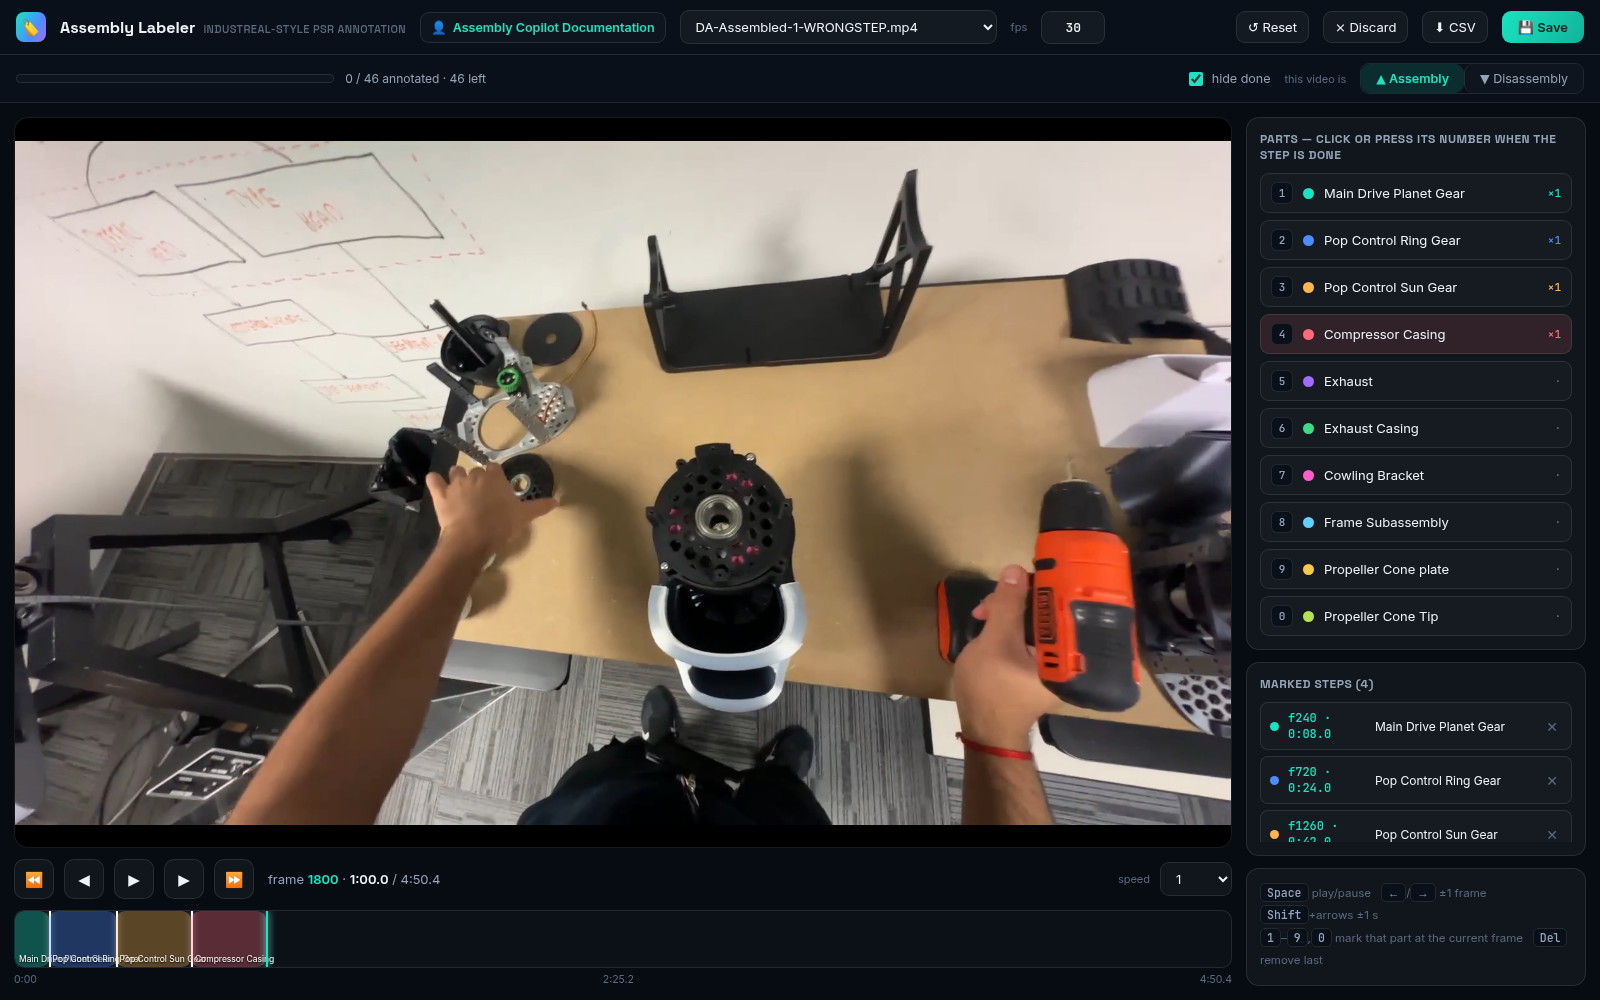
\includegraphics[width=0.94\textwidth]{labeler_loaded.png}
\caption{Labeling application with a recording loaded. The operator can review
the video and mark procedure completion events against the part list.}
\label{fig:labeler}
\end{figure}

The tool produces a completion-label CSV, a segment CSV, and a JSON
representation. These artifacts are converted into the frame-wise labels used
for feature extraction, training, and replay visualization. Labeling the
completion event rather than only naming a clip makes the data useful for
temporal segmentation and step-transition evaluation.

\section{Label Semantics and Derived Training Data}

Each completion mark represents the point at which the annotator judged that a
part installation or removal had finished. The downstream preparation scripts
turn these sparse transition events into dense frame-wise targets: frames before
and after a transition receive the corresponding procedure-state label, and
frames in which no modeled action is active receive the background label. This
conversion is what allows the temporal model to learn both the action interval
and the boundary between adjacent steps.

The project retained the raw completion labels, the derived segments, and the
model-ready labels as separate artifacts. Keeping these levels distinct made it
possible to correct an annotation without losing the source decision, compare
different boundary interpretations, and reproduce the same feature/label
alignment during offline and online evaluation.

\section{Dataset Preparation and Split Discipline}

The production library was organized by recording rather than by randomly
sampling individual frames. Feature extraction created one fused feature
sequence per recording, and the train/test split was applied at the recording
level. This avoids placing neighboring frames from the same take in both
partitions. The current operator population is not subject-disjoint, which is
recorded as a limitation rather than hidden by a random frame split.

\section{Assembly Step Vocabulary}

\begin{table}[H]
\centering
\small
\begin{tabularx}{\textwidth}{@{}p{0.10\textwidth}p{0.43\textwidth}X@{}}
\toprule
\textbf{Key} & \textbf{Part} & \textbf{Assembly / disassembly label IDs} \\
\midrule
1 & Main Drive Planet Gear & Install 3 / remove 5 \\
2 & Pop Control Ring Gear & Install 6 / remove 8 \\
3 & Pop Control Sun Gear & Install 9 / remove 11 \\
4 & Compressor Casing & Install 12 / remove 14 \\
5 & Exhaust & Install 15 / remove 17 \\
6 & Exhaust Casing & Install 18 / remove 20 \\
7 & Cowling Bracket & Install 21 / remove 23 \\
8 & Frame Subassembly & Install 24 / remove 26 \\
9 & Propeller Cone plate & Install 27 / remove 29 \\
0 & Propeller Cone Tip & Install 30 / remove 32 \\
\bottomrule
\end{tabularx}
\caption{Procedure vocabulary used by the labeling application and model
dataset.}
\label{tab:step-vocabulary}
\end{table}

\section{Stress Variants}

Normal recordings alone do not test whether the system has learned the
procedure or has memorized a familiar order. The project therefore created
stress variants including scrambled order, reversed procedure, partial
recordings, and wrong-step cases. These assets support controlled checks for
order robustness, cold starts, and behavior when the observed action is
inconsistent with the expected sequence.

The scrambled condition is particularly important because it breaks the
assumption that the next part can be inferred from a fixed nominal order. A
reversed recording tests directionality, a partial recording tests initialization
away from the beginning of a procedure, and a wrong-step recording tests how
the application communicates activity that conflicts with the expected state.
Together these variants distinguish visual recognition from simple procedure
position tracking.

\chapter{Model Development and Results}

\section{Research Progression on IndustReal}

IndustReal was used as the controlled research setting for comparing temporal
heads, backbones, decoding, and feature fusion. The progression below records
the measured recognition results. Acc is frame accuracy, Edit is edit score,
and F1@50 is segmental F1 at an overlap threshold of 50 percent.

\begin{table}[H]
\centering
\scriptsize
\begin{tabularx}{\textwidth}{@{}Xrrr@{}}
\toprule
\textbf{Configuration} & \textbf{Acc} & \textbf{Edit} & \textbf{F1@50} \\
\midrule
v1 Huge-K710 + ASFormer (baseline) & 73.3 & 68.8 & 56.3 \\
v1 + Viterbi & 73.4 & 74.2 & 62.2 \\
v2 SSv2-giant + ASFormer + Viterbi & 74.0 & 77.3 & 66.5 \\
v2 SSv2-giant + DiffAct & 74.4 & 79.6 & 68.9 \\
Fusion (giant + IV2-B14) + ASFormer + Viterbi & 75.7 & 77.6 & 68.2 \\
\textbf{v4 Fusion + DiffAct --- best} & \textbf{84.21} & \textbf{87.19} & \textbf{79.50} \\
v4 + SAM3 enrichment & 74.9 & 79.5 & 70.1 \\
\bottomrule
\end{tabularx}
\caption{IndustReal research progression.}
\label{tab:industreal-results}
\end{table}

\section{Iteration-by-Iteration Interpretation}

The table is a development sequence rather than a list of unrelated
experiments. Each iteration answered a specific question about the system.

\begin{enumerate}
    \item \textbf{v1: VideoMAEv2-Huge with ASFormer.} This established the
    baseline for frame recognition and temporal segmentation. Its accuracy was
    usable, but the lower Edit and F1@50 scores showed that the predicted
    segments were not yet sufficiently aligned or stable at procedure
    boundaries.
    \item \textbf{v1 with Viterbi decoding.} The visual representation was
    unchanged; only the sequence decoding was improved. Edit increased from
    68.8 to 74.2 and F1@50 from 56.3 to 62.2. This demonstrated that temporal
    consistency was an important source of improvement, not just a larger
    backbone.
    \item \textbf{v2: SSv2-giant features.} Moving to the stronger giant
    representation raised accuracy and improved the overall feature quality.
    With ASFormer and Viterbi, the system reached 74.0 accuracy, 77.3 Edit,
    and 66.5 F1@50.
    \item \textbf{v2 with DiffAct.} Replacing the temporal head produced a
    further improvement in segment quality: F1@50 increased to 68.9 and Edit
    to 79.6. This identified DiffAct as the strongest offline temporal head in
    the tested progression.
    \item \textbf{Fusion of motion and appearance.} VideoMAEv2-giant and
    InternVideo2-B14 contributed different evidence. The fused representation
    with ASFormer and Viterbi reached 75.7 accuracy and 77.6 Edit, although its
    F1@50 did not exceed the v2 DiffAct result. This showed that feature fusion
    and temporal modeling had to be selected together.
    \item \textbf{v4: Fusion with DiffAct.} Combining the best representation
    with the strongest tested offline temporal head produced the clear best
    result: 84.21 accuracy, 87.19 Edit, and 79.50 F1@50. This became the
    reference architecture and feature recipe before the project moved to its
    own engine-model recordings.
    \item \textbf{SAM3 enrichment.} Adding segmentation-based enrichment did
    not improve the recognition result; the measured configuration fell to
    74.9 accuracy, 79.5 Edit, and 70.1 F1@50. SAM3 therefore remained an
    exploratory object/mask branch rather than a replacement for the temporal
    recognition path.
\end{enumerate}

\section{What the IndustReal Results Established}

The experiments established three practical conclusions. First, motion and
appearance information were complementary: motion described how the operator
was acting, while appearance helped distinguish visually similar parts and
contexts. Second, temporal decoding materially affected the quality of
procedure boundaries; a frame-accurate classifier was not sufficient by
itself. Third, the strongest offline result was not automatically the correct
deployment model. DiffAct benefited from sequence context that is unavailable
at the moment a live decision is required.

The research also exposed the limits of using a recognition model as a
correctness inspector. In the reported ablation, VideoMAE-only configurations
had 0\% incorrect-install recall, while the giant plus InternVideo2-B14 fusion
produced the first non-zero recall at 10.1\%. That improvement was useful
evidence that appearance fusion could help identify abnormal actions, but it
was not sufficient to claim reliable visual verification. The live
demonstrator therefore focuses on procedure-step recognition and flags
sequence deviations for review rather than certifying installation quality.

\section{Decision Before Moving to the Own Dataset}

\begin{table}[H]
\centering
\small
\begin{tabularx}{\textwidth}{@{}p{0.34\textwidth}X@{}}
\toprule
\textbf{Research decision} & \textbf{How it shaped the next phase} \\
\midrule
Retain dual-stream features & The engine-model pipeline used the complementary
motion and appearance encoders rather than reverting to a single backbone. \\
Use v4 as the offline reference & The fused representation plus DiffAct
provided the upper-bound reference for the in-house dataset. \\
Do not deploy DiffAct unchanged & Its offline context requirement led to a
causal temporal head for live inference. \\
Keep decoding explicit & Fixed-lag sequence commitment was retained so that
the interface would report stable steps rather than every transient class
change. \\
Treat correctness as a separate problem & The first deployment target remained
step recognition, out-of-order detection, and procedure-state presentation. \\
\bottomrule
\end{tabularx}
\caption{Research decisions carried into the engine-model development phase.}
\label{tab:research-decisions}
\end{table}

\section{Evaluation Metrics and Selection Logic}

Accuracy measures the proportion of correctly classified frame positions. Edit
score measures the similarity of the predicted and reference action order after
collapsing repeated labels, so it is sensitive to extra, missing, or misplaced
segments. F1@50 measures whether predicted action segments overlap reference
segments by at least 50\%. The progression was selected using all three: a
model was not considered better merely because it improved frame accuracy if
its procedure boundaries became less reliable.

\section{Engine-Model Dataset Results}

\begin{table}[H]
\centering
\small
\begin{tabularx}{\textwidth}{@{}Xrrr@{}}
\toprule
\textbf{Configuration} & \textbf{Acc} & \textbf{Edit} & \textbf{F1@50} \\
\midrule
v4 Fusion + DiffAct (offline) & 96.21 & 97.33 & 97.51 \\
Baseline (online) & 92.96 & 75.65 & 81.36 \\
\textbf{Final Online V1} & \textbf{94.12} & \textbf{84.45} & \textbf{89.50} \\
\bottomrule
\end{tabularx}
\caption{Engine-model dataset results supplied for the project evaluation.}
\label{tab:engine-results}
\end{table}

The offline result is a useful upper-bound reference: it benefits from
sequence context that is unavailable at deployment time. Final Online V1
improves substantially over the online baseline in temporal quality while
retaining strong frame accuracy. The gap between offline and online results is
expected and is the reason the deployment metrics are reported separately.

\section{From Offline Models to Causal Inference}

The causal temporal convolutional network uses nine dilated blocks with 128
feature maps and approximately 875 thousand trainable parameters. Its
receptive field is approximately 205 seconds, but its computation is causal:
the output at time $t$ depends on the current and previous feature sequence,
not on future frames. This gives the model enough history to understand
procedure context while preserving the online constraint.

The final class set contains eleven classes: the ten modeled parts and a
background state. The network generates class scores for each feature update.
The fixed-lag decoder then converts those scores into stable committed steps for
the application.

\section{Robustness Iteration and Acceptance Gate}

The deployed checkpoint, \texttt{robust\_v1}, was trained with normal recordings,
mid-start crops, and scrambled-order variants. The project acceptance gate
measured both normal behavior and the harder scrambled-order behavior.

\begin{table}[H]
\centering
\small
\begin{tabularx}{\textwidth}{@{}p{0.34\textwidth}rrrX@{}}
\toprule
\textbf{Checkpoint / run} & \textbf{Normal} & \textbf{Scrambled} &
\textbf{Cold start} & \textbf{Decision} \\
\midrule
Previous baseline & 93.45\% & 72.58\% & 19.2 s & Reference only \\
Fine-tune A & 92.39\% & 91.40\% & --- & Rejected: normal floor \\
Fine-tune A2 & 92.95\% & 88.84\% & --- & Passed interim check; not selected \\
\texttt{robust\_v1} & 93.06\% & 90.57\% & 0.2 s & Deployed checkpoint \\
\bottomrule
\end{tabularx}
\caption{Robustness iteration and deployment selection.}
\label{tab:robustness-gate}
\end{table}

\section{Checkpoint-to-Application Handoff}

Once the checkpoint passed the gate, the model was not treated as an isolated
file. The feature-extraction path, class vocabulary, decoder lag, and service
state all had to remain aligned. The replay service loads the checkpoint and
runs it over a complete recording; the live service loads the same checkpoint
and updates it incrementally as new clips arrive. The shared state contract
then allows the browser and HoloLens clients to present the result without
duplicating model logic.

\begin{table}[H]
\centering
\small
\begin{tabularx}{\textwidth}{@{}p{0.33\textwidth}X@{}}
\toprule
\textbf{Handoff step} & \textbf{Engineering purpose} \\
\midrule
Prepare or compute fused features & Guarantee the same clip length, sampling
rate, normalization, and feature ordering used during training. \\
Load the causal checkpoint & Use the selected temporal head and class order
consistently in replay and live services. \\
Run fixed-lag commitment & Convert repeated model scores into stable step
transitions and measurable delay. \\
Publish procedure state & Give presentation clients current step, progress,
and attention information through one interface. \\
\bottomrule
\end{tabularx}
\caption{The engineering handoff from a trained checkpoint to the
demonstration.}
\label{tab:checkpoint-handoff}
\end{table}

\section{Optional Visual Enrichment}

SAM3-based enrichment was explored as a supporting visual branch for masks and
part inventory. It was useful for investigating object-level cues, but it did
not replace the temporal recognition path and did not become the basis of the
deployed live checkpoint. The separation keeps the demonstrated system focused:
the primary model recognizes procedure state from the egocentric sequence.

\chapter{Applications and Demonstration}
\section{Replay Inference}
The replay application provides a repeatable way to inspect the system. A recorded
video is submitted to the service, processed through the same causal model and
decoder used by the live path, and displayed with the predicted current step.
The interface also shows the procedure list and a human-versus-AI timeline so
that a reviewer can compare recognition quality, transition timing, and
out-of-order behavior on the same recording.
\begin{figure}[H]
\centering
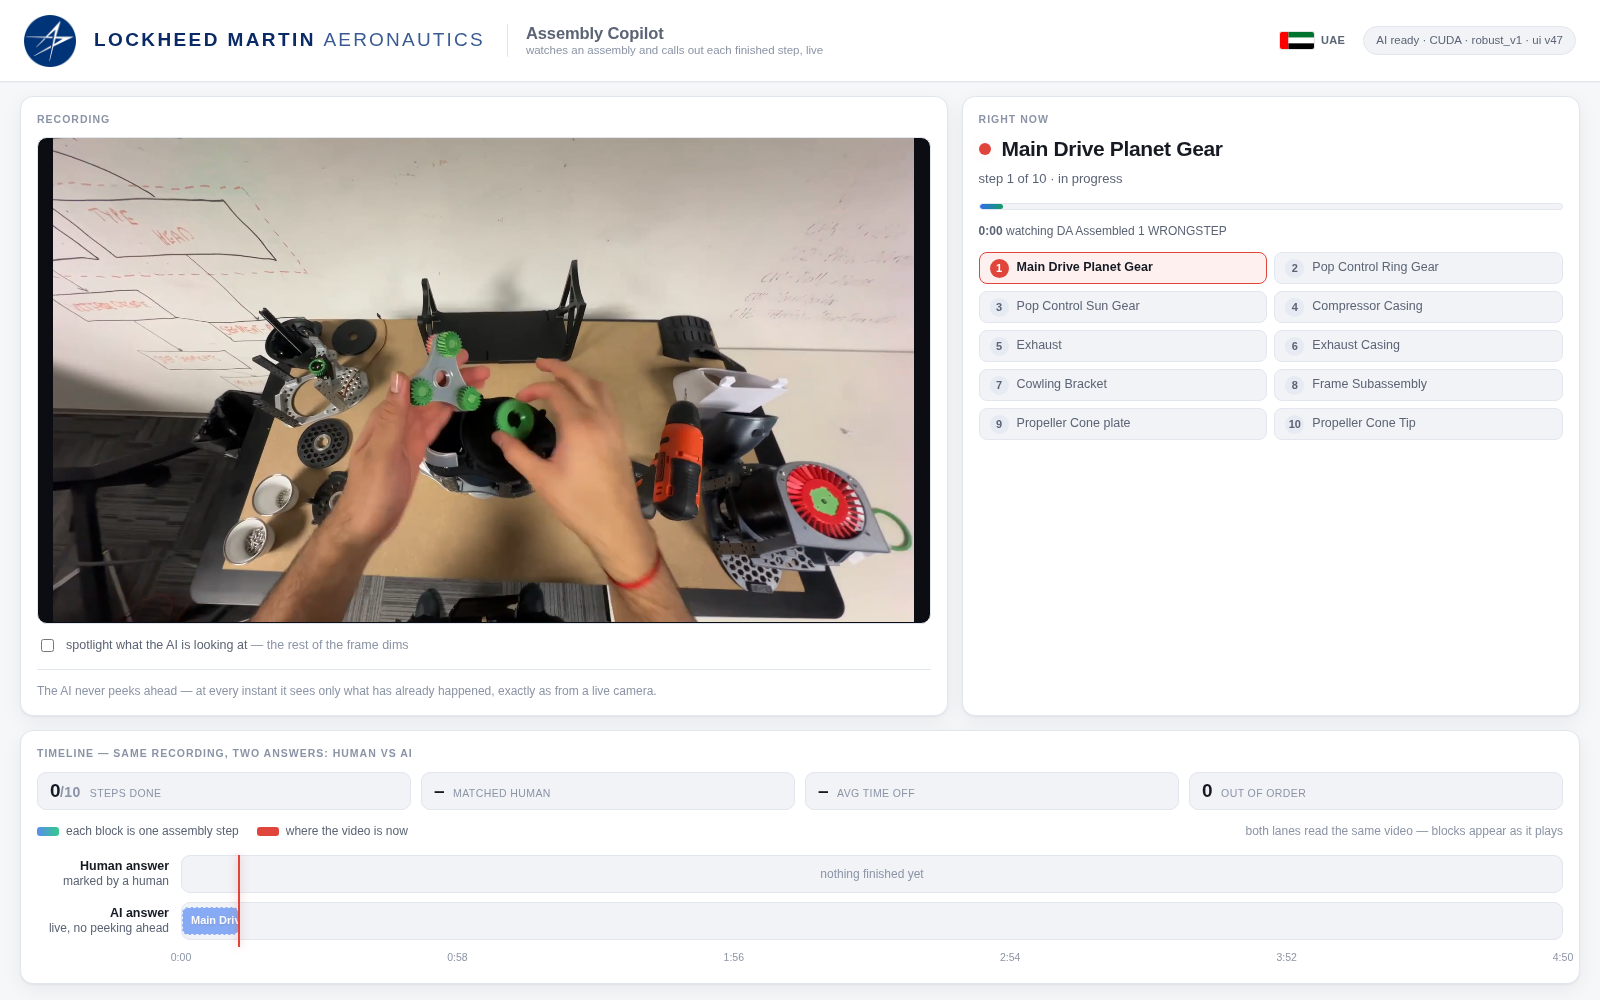
\includegraphics[width=0.94\textwidth]{replay_inference_loaded.png}
\caption{Replay inference interface with a project recording loaded.}
\label{fig:replay}
\end{figure}
\section{Live Inference Path}
The live demonstration receives camera frames over the recording/WebRTC path.
The service derives the model's 10 fps input, maintains a rolling clip buffer,
computes features, updates the causal model, and publishes the current state.
This path exercises transport, frame sampling, feature extraction, temporal
state, decoding, and presentation simultaneously. The measured implementation
runs at approximately 1.14 times playback speed, with an end-to-end
announcement delay of approximately 2.84 seconds.

\section{Live State and Step Progression}

The live service publishes the current committed label, procedure direction,
step progress, and attention status. A prediction that changes for one update
does not immediately change the displayed step; the fixed-lag decoder must
first commit the transition. This is why the interface can update frequently
without making the operator watch a flickering sequence of competing labels.

\section{HoloLens Overlay}
The wearable presentation is implemented as a separate Unity Universal Windows
Platform application for HoloLens. The current project uses Unity 2020.3.28f1
with Microsoft Mixed Reality Toolkit/OpenXR components. The trained model
remains on the inference service; the Unity client polls the service state and
renders the result as a movable, resizable 2D overlay.
\begin{figure}[H]
\centering
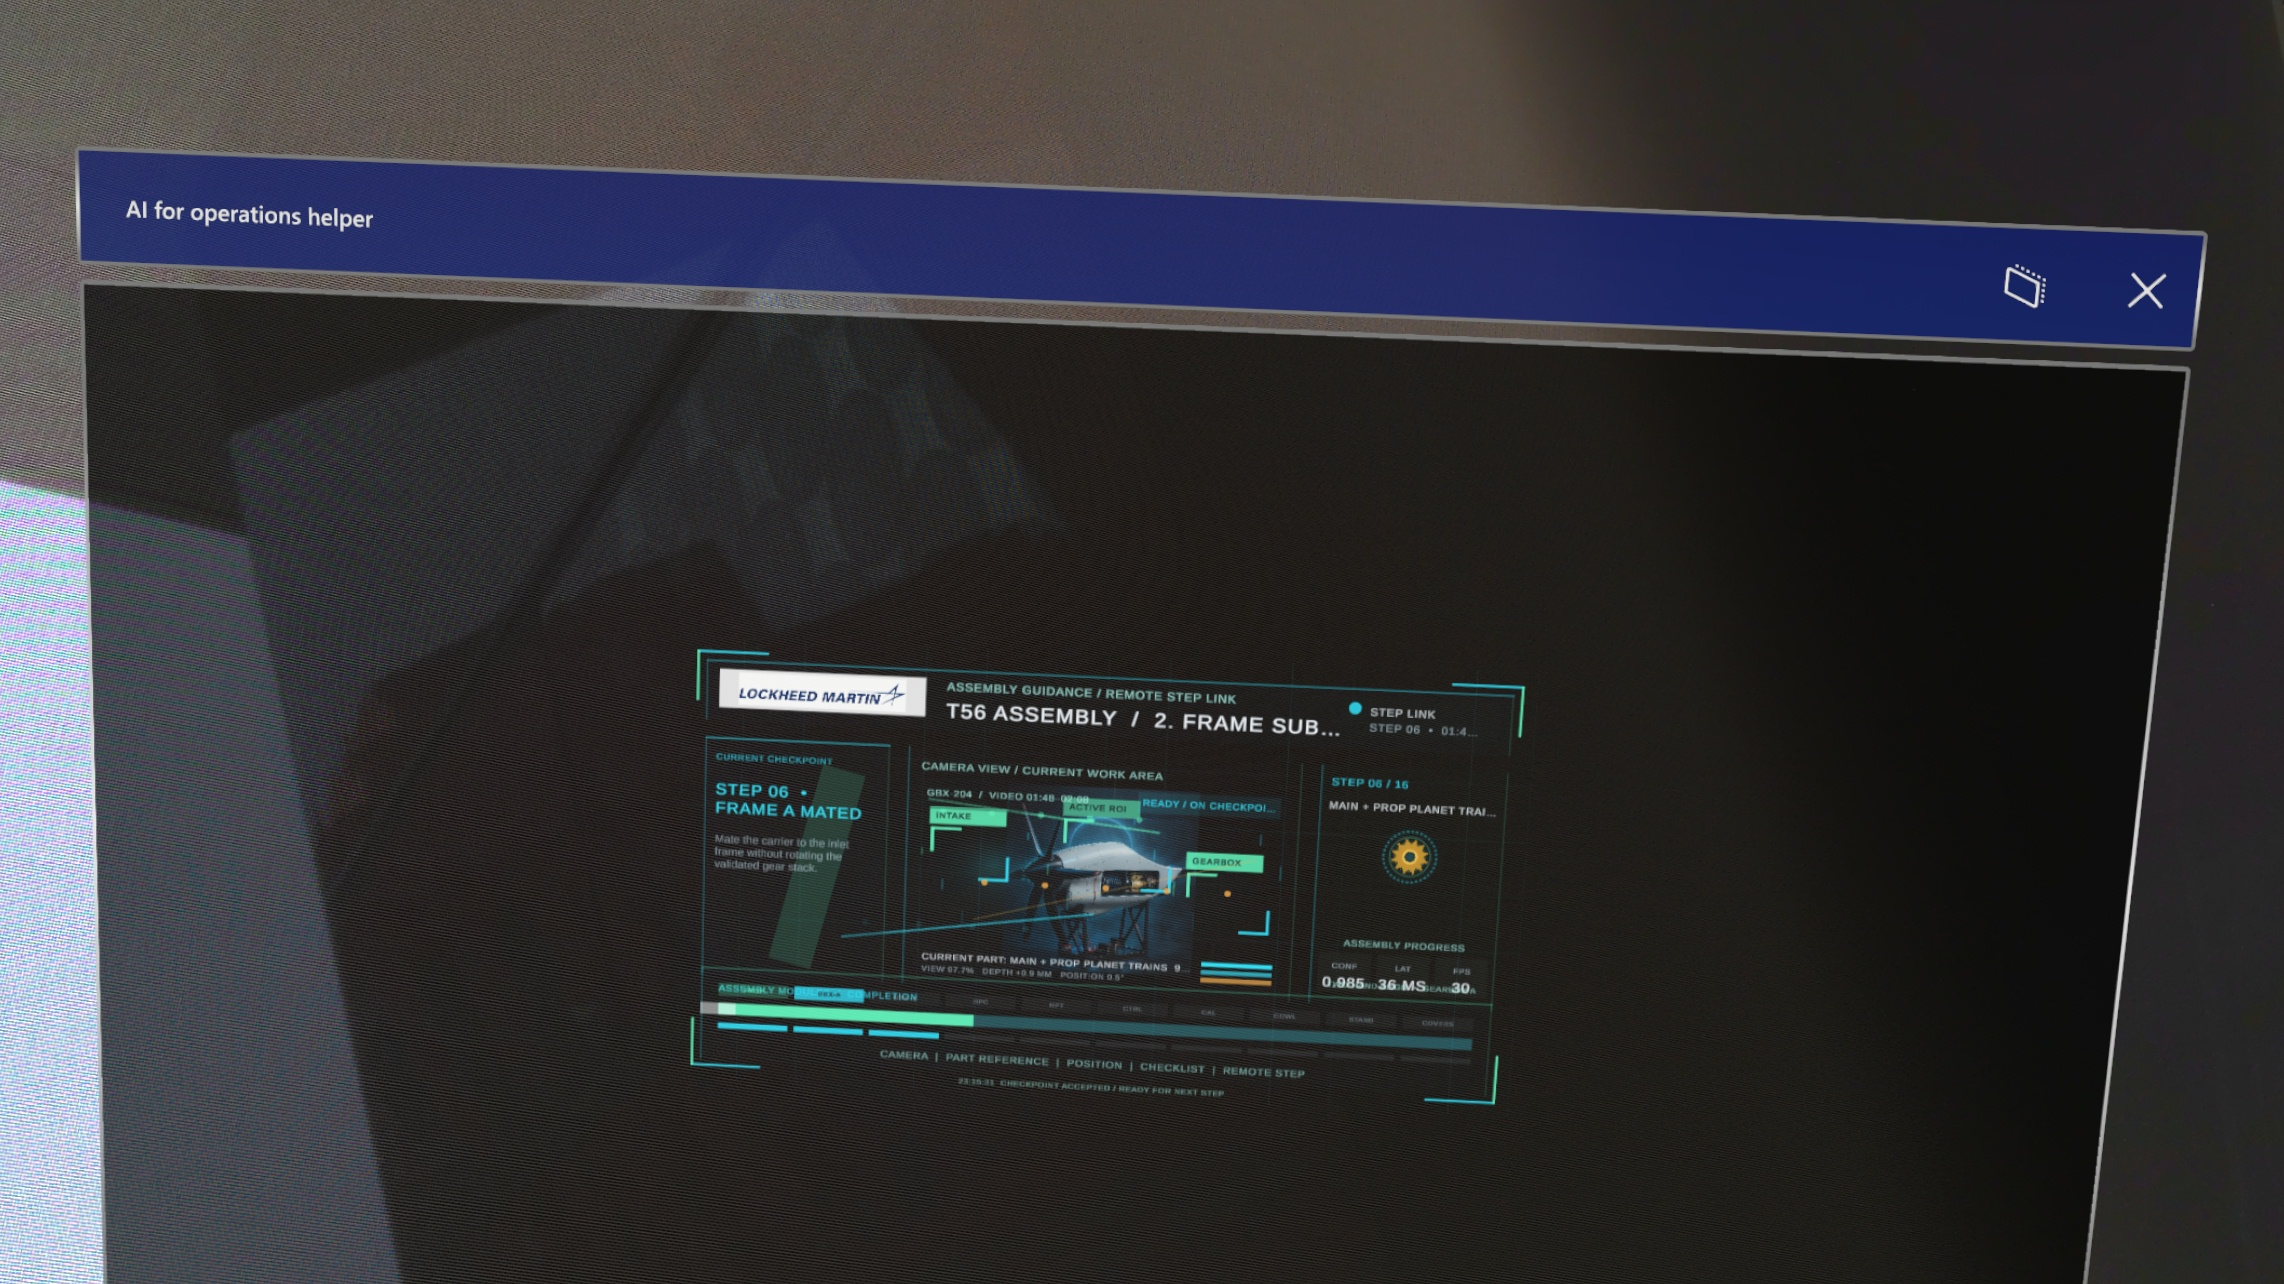
\includegraphics[width=0.94\textwidth]{hololens_overlay.jpg}
\caption{HoloLens overlay demonstration showing procedure guidance and current state.}
\label{fig:hololens}
\end{figure}

The HoloLens project is a separate Unity Universal Windows Platform client
using Unity 2020.3.28f1 with Microsoft Mixed Reality Toolkit/OpenXR components.
The trained model remains on the inference service. The Unity client polls the
service state and renders it as a movable, resizable 2D overlay. The current
implementation is screen-space rather than spatially anchored to a physical
part; spatial anchors, part localization, and reference-based geometry checks
are future extensions.

\section{Presentation of the Result}
The user-facing state includes:
\begin{itemize}
    \item the current or most recently committed step;
    \item the ordered procedure list and completion status;
    \item an indication when observed activity is out of order or requires
    attention;
    \item a timeline for comparing human labels with AI commitments.
\end{itemize}

\section{What the Demonstration Proves}

The demonstration proves that the research result has been connected to a
complete application path. It does not prove that every assembly fault can be
detected or that the current screen-space overlay is ready for production use.
The evidence is strongest for the following claims: the system can process
egocentric recordings, maintain a causal running estimate, stabilize its
announcements, display procedure progress, and expose a usable interface for
review or wearable presentation.

\chapter{Validation, Limitations, and Next Steps}

\section{What Has Been Demonstrated}

The project has progressed beyond a model-only experiment. The completed chain
includes a repeatable egocentric recording workflow, a browser-based labeling
application with structured exports, a curated engine-model dataset and
generated stress variants, controlled IndustReal and engine-model evaluation, a
causal live inference service with fixed-lag step commitment, and replay, live,
and HoloLens presentation paths.

The strongest supplied engine-model offline result is 96.21\% accuracy,
97.33 edit score, and 97.51 F1@50. The final online result is 94.12\%,
84.45 edit score, and 89.50 F1@50. The deployed robustness checkpoint reaches
90.57\% on the scrambled-order stress condition and starts producing output
after approximately 0.2 seconds in the reported gate.

\section{Current Limitations}

\begin{enumerate}
    \item The current held-out split is recording-disjoint but not
    subject-disjoint; performance on new operators is not yet isolated.
    \item The model recognizes procedure-step evidence. It is not a complete
    visual inspection system and should not be interpreted as proof that a
    part is installed correctly.
    \item The live output has a deliberate delay from clip context and decoder
    stabilization.
    \item The wearable client currently presents a screen-space overlay rather
    than a spatially anchored instruction at the physical part.
    \item The learned vocabulary covers ten modeled parts, while a presentation
    or overlay may show additional workflow or verification states. These
    should not be confused with learned recognition classes.
    \item The feature encoders are computationally substantial. A production
    deployment would need a defined edge, workstation, or network-inference
    architecture and an operational monitoring plan.
\end{enumerate}

\section{Recommended Next Steps}

\begin{enumerate}
    \item Collect more operators, lighting conditions, camera placements, and
    procedure variations; introduce a subject-disjoint evaluation split.
    \item Expand labels beyond completion events to include wrong part, omitted
    step, rework, hesitation, and verification outcomes.
    \item Improve the live path by measuring per-stage latency, testing
    hardware-aware optimization, and defining an acceptable alert-delay
    envelope with end users.
    \item Add spatial registration and part localization only where the
    operator workflow benefits from an anchored visual cue.
    \item Establish a production evaluation protocol with confidence
    thresholds, false-alert review, model/version traceability, and approved
    human decision points.
\end{enumerate}

\section{Reproducibility and Dependencies}

The repository contains the model code, dataset preparation scripts, recorded
assets, checkpoint, and the replay/live services. The software path is based on
Python and PyTorch, with FastAPI/Uvicorn for the services and standard video
processing utilities for frame handling. CUDA is used when available; CPU
execution is supported for inspection but is not the intended performance
configuration for the full encoder path. The HoloLens presentation is a
separate Unity UWP project using MRTK/OpenXR. The reproducibility guide in the
project defines the staged sequence: prepare features and labels, generate
stress data, train, run the acceptance gate, and launch the served applications.

\chapter{Conclusion}

Assembly Copilot demonstrates an end-to-end approach to procedure-step
recognition from egocentric video. The work combined research experimentation,
purpose-built data collection and labeling, temporal model iteration, causal
online decoding, and application integration. The result is a working
demonstrator that can process recorded or live video, identify stable procedure
steps, expose deviations for review, and present the current state through a
wearable interface.

The most important engineering outcome is the transition from a strong offline
recognition result to a bounded live system. The deployed design accepts a
small, explicit delay to obtain stable commitments, while remaining causal and
close to real time. With broader data, subject-disjoint validation, stronger
error labels, and spatially registered guidance, the same foundation can be
developed into a more complete assembly-assistance capability.

\chapter*{References}
\addcontentsline{toc}{chapter}{References}

\begin{thebibliography}{99}
\bibitem{industreal} F. Ragusa et al. IndustReal: A Dataset and Benchmark for Industrial Procedure Understanding, 2023.
\bibitem{videomae} M. Wang et al. VideoMAE V2: Scaling Video Masked Autoencoders with Dual Masking, CVPR, 2023.
\bibitem{internvideo2} Y. Wang et al. InternVideo2: Scaling Video Foundation Models for Multimodal Video Understanding, 2024.
\bibitem{asformer} F. Yi et al. ASFormer: Transformer for Action Segmentation, BMVC, 2021.
\bibitem{diffact} M. Nawhal et al. DiffAct: Context-Aware Diffusion Actions for Online Action Detection, 2024.
\bibitem{sam3} Meta AI. Segment Anything Model 3, project documentation, 2025.
\bibitem{copilotrepo} Assembly Copilot Project. README, REPRODUCING.md, and model/application source, internal repository, 2026.
\bibitem{labeltools} Assembly Copilot Project. Assembly Video Recorder and Assembly Video Labeler, internal tools, 2026.
\bibitem{hololens} Assembly Copilot Project. HoloLens overlay application and integration notes, internal application, 2026.
\end{thebibliography}


\end{document}
